%%
%% 9April2008.tex
%% 
%% Made by Alex Nelson
%% Login   <alex@tomato>
%% 
%% Started on  Fri Dec 19 22:16:02 2008 Alex Nelson
%% Last update Fri Dec 19 22:16:02 2008 Alex Nelson
%%
\subsection{Convergence of Fourier Series}
Now let us examine another definition of piecewise
continuous~\cite{textbook}:
\begin{defn}
If $f$ is piecewise continuous\index{Continuity!Piecewise Continuous} on $(a,b)$, then $f$ is
continuous except ``perhaps'' at finitely many jumps
(``discontinuities''); if $f$ is piecewise continuous on
$\mathbb{R}$, then it is piecewise continuous for all
$-\infty<a<b<\infty$.
\end{defn}
But it is worthy of note that if $f$ is continuous, it has
``nicer'' Fourier coefficients than if $f$ were merely
piecewise continuous. What are ``nice'' and ``mean'' Fourier
coefficients? Well, how quickly they decay determines how
many terms we need to get a good approximation. If the
fourier coefficients decay quickly (so $c_{n}\to 0$
quickly), then the Fourier coefficients are ``nicer''.

\begin{prop}
If $f$ is continuous and piecewise smooth on $\mathbb{R}$,
then $f$ is continuous and $f'$ is piecewise continuous.
\end{prop}
\begin{proof}
How can we make this claim? Well recall that we defined
piecewise smooth to be when both $f$ and $f'$ are piecewise
continuous. But we have the additional property that $f$ is
continuous, which is stronger than piecewise continuous. So
if $f$ is continuous and piecewise smooth, it is equivalent
to saying that $f'$ is piecewise continuous and $f$ is
continuous (since continuous is stronger than piecewise
continuous, we call it the stronger of the two). All
continuous functions are also piecewise continuous, so it is
more strict a condition to be continuous.
\end{proof}

Now we should probably review a few definitions.

\begin{defn}
Consider a series of functions
\begin{equation*}
\sum_{n}g_{n}(x) = g(x).
\end{equation*}
If for each $x\in D\subseteq\mathbb{R}$ (each $x$ in the
domain which could be the entire real line), we say the
series \textbf{converges absolutely}\index{Convergence!Series, Absolutely} if
$\sum|g_{n}(x)|$ converges.
\end{defn}

\begin{defn}
Consider a series of functions
\begin{equation*}
\sum_{n}g_{n}(x) = g(x).
\end{equation*}
We say that the series \textbf{converges uniformly}\index{Convergence!Series, Uniformly}
if for each $\varepsilon>0$ there is some $N\in\mathbb{N}$
such that
\begin{equation}
|g(x) - \sum^{M}_{n=0}g_{n}(x)|<\varepsilon,\qquad\forall M\geq N.
\end{equation}
\end{defn}
\marginpar{Weierstrass M-test}There is an excellent test to
see if a series converges or not. The idea is to take a
series that we know converges, but is term for term bigger
than the series we are examining. If the series we are
testing is term for term smaller than something that
converges, then we know the series we are testing
converges. 

The standard ``tricks'' to do this is to use bounds for the
series. Typically we want to make the numerator (the top
part of the fraction) as big as possible, and the
denominator as small as possible. So we typically bound
$\sin(x)\leq 1$ and $\cos(x)\leq 1$. There are other tricks
that perhaps we will see later on.

This test which says ``If term for term a series in question
is less than a series known to converge, then the series in
question converges'' is known in the mathematical community
as \textbf{Weierstrass M-test}\index{Convergence!M-Test}\index{Weierstrass M-test}.
More specifically, if we have a series that is known to converge
\begin{equation}
\sum_{n}M_{n} = M
\end{equation}
and if we need to test a given series
\begin{equation*}
\sum_{n}g_{n}(x)
\end{equation*}
\marginpar{M-test guarantees both \emph{uniform} and \emph{absolute} convergence}and also suppose that term for term $|g_n(x)|\leq M_n$ for
all $x\in D$ (where D is the domain of the functions), then
\begin{equation}
\sum g_{n}(x)\leq M
\end{equation}
converges absolutely and uniformly.

\begin{ex}
Recall our Fourier series expansion of the triangle wave
\begin{equation}
f(\theta) = \frac{\pi}{2} -
\frac{4}{\pi}\sum^{\infty}_{n=1}\frac{\cos[(2n-1)\theta]}{(2n-1)^2}
\end{equation}
By the Weierstrass M-test, we have
\begin{equation}
\left|\frac{\cos[(2n-1)\theta]}{(2n-1)^{2}}\right|\leq\frac{1}{(2n-1)^2}
\end{equation}
for all $\theta$. If we are also uncertain, we know
\begin{equation}
\frac{1}{(2n-1)^{2}}\leq \frac{1}{n^{2}}
\end{equation}
for all $n\in\mathbb{N}$ and we know that the series
\begin{equation}
\sum_{n=1}\frac{1}{n^{2}}=\frac{\pi^2}{9}.
\end{equation}
Thus by the Weierstrass M-test, the Fourier series converges
uniformly and absolutely.
\end{ex}

\begin{thm}\label{thm:9April2008:thm2.5}
If $f$ is a $2\pi$-periodic, continuous and piecewise smooth
function, then the Fourier series of $f$ converges to $f$
absolutely and uniformly.
\end{thm}

The consequence of Theorem \eqref{thm:9April2008:thm2.5} is
that if $f$ is equal to its Fourier series, then
\begin{equation}
\int^{b}_{a}f(\theta)d\theta =
\sum_{n}\int^{b}_{a}c_{n}e^{in\theta}d\theta
\end{equation}
for any $-\infty<a<b<\infty$.

\begin{sketch}
We need to show that
\begin{equation}
\sum^{\infty}_{n=-\infty}|c_{n}|<\infty,
\end{equation}
then apply the Weierstrass M-test to get absolute and
uniform convergence. We need to show three things: 1)
Fourier coefficient of $f'$ (denoted $c_{n}'$) is
$c_{n}=-ic_{n}'/n$; 2) the Bessel inequality for $f'$ says
$\sum|c_{n}'|^2\leq(1/2\pi)\int^{\pi}_{-\pi}|f'(\theta)|^{2}d\theta$;
3) the Cauchy-Schwarz inequality, which says
$\sum|\alpha_n\beta_n|\leq(\sum|\alpha_n|)^{1/2}(\sum|\beta_n|)^{1/2}$. Thus
we find
\begin{subequations}
\begin{align}
\sum|c_{n}| &= \sum^{\infty}_{n=-\infty}
\left|\frac{c_{n}'}{n}\right|+|c_{0}| \\
&\leq\left(\sum_{n\neq0}\frac{1}{n^{2}}\right)^{1/2}\left(\sum_{n\neq0}|c_{n}'|^{2}\right)^{1/2}
+ |c_0| \\
&<+\infty
\end{align}
\end{subequations}
We can plug in the Bessel inequality to find
\begin{equation}
\sum|c_{n}|\leq\left(\frac{\pi}{\sqrt{6}}\right)\left(\frac{1}{2\pi}\int^{\pi}_{-\pi}|f'(\theta)|^{2}d\theta\right)+|c_{0}|
\end{equation}
On that note, we will end our sketch of the proof.
\end{sketch}

We will need to examine two ideas before we can perform our
proof. One is the Fourier coefficients of the derivative of
a function. The other is the Cauchy-Schwarz inequality,
which proves itself useful time and time again in mathematics.

\subsection{Termwise Integration of Fourier Series}

We still haven't really answered the question ``When does
the Fourier series converge, and to what?'' We saw for
$2\pi$-periodic, continuous and piecewise smooth functions
that the Fourier series converges absolutely and uniformly
(and in a remarkably handwavy way, anything that is $C^{1}$
would converge absolutely and uniformly too). So let us now
try to examine all the details of when and what does the
Fourier series converge to. We will let
\begin{equation}
F(\theta) = \int^{\theta}_{0}f(\phi)d\phi.
\end{equation}

\begin{assume}
Let $f$ be $2\pi$-periodic and piecewise continuous on $\mathbb{R}$.
\end{assume}

Now if $f$ has an antiderivative $\widetilde{F}$, then 
\begin{equation}
F(\theta) = \widetilde{F}(\theta) - \widetilde{F}(0)
\end{equation}
by the fundamental theorem of calculus. So we can make a
number of additional claims\begin{enumerate}[a)]
\item $F$ is continuous, i.e. $F(\theta^{+})=F(\theta^{-})$
  for all $\theta$
\item $F$ is piecewise smooth on $\mathbb{R}$, and $f$ is
  piecewise continuous. We have
  $F'(\theta)=(d/d\theta)\int^{\theta}_{0}f(\phi)d\phi=f(\theta)$
  where $f(\theta)$ is continuous.
\item (Assumption for this step:
  $c_{0}=a_{0}/2=(1/2\pi)\int^{\pi}_{-\pi}f(\theta)d\theta=0$)
  $F$ is $2\pi$-periodic
  (i.e. $F(\theta+2\pi)-F(\theta)=\int^{\theta+2\pi}_{\theta}f(\phi)d\phi=\int^{\pi}_{-\pi}f(\phi)d\phi=0$
  by our assumption. 
\end{enumerate}
Let the Fourier coefficients of $F$ be $C_n$, $A_n$ and
$B_n$, and the coefficients for $F'=f$ be $c_n$, $a_n$ and
$b_n$. So we know
\begin{equation}
c_{n}=C_{n}' = inC_{n}\Rightarrow C_{n}=\frac{c_n}{in}
\end{equation}
and similarly
\begin{equation}
A_{n} = -\frac{b_n}{n},\qquad B_n=\frac{a_n}{n}
\end{equation}
Thus the Fourier series of $F$ is
\begin{subequations}
\begin{align}
F(\theta) &= C_{0} +
\sum_{n\neq0}\frac{c_n}{in}e^{in\theta}\\
&=\frac{1}{2}A_{0} + \sum_{n=1}\left(\frac{-b_n}{n}\cos(n\theta)+\frac{a_n}{n}\sin(n\theta)\right)
\end{align}
\end{subequations}
where $C_0=A_0/2=(1/2\pi)\int^{\pi}_{-\pi}F(\theta)d\theta$.

For any $2\pi$-periodic , piecewise continuous function $f$,
then it can be expanded into a Fourier Series
\begin{equation}
f(\theta) = c_0 + \sum_{n\neq0}c_{n}e^{in\theta}
\end{equation}
where $c_0$ may be zero. We may define
$g(\theta)=f(\theta)-c_0$ which satisfy conditions (a), (b),
and (c) outlined above. So
\begin{subequations}
\begin{align}
\int^{\theta}_{0}(f(\phi)-c_{0})d\phi &= C_{0} +
\sum_{n\neq0}C_{n}e^{in\theta}\\
&= C_{0}+\sum_{n\neq0}\frac{c_{n}}{in}e^{in\theta}
\end{align}
\end{subequations}
So $\int^{\theta}_{0}(f(\phi)-c_0)d\phi =
\int^{\theta}_{0}f(\phi)d\phi - c_0\theta =
F(\theta)-c_0\theta$ and
\begin{equation}
C_{0} =
\frac{1}{2\pi}\int^{\pi}_{-\pi}(F(\theta)-c_{0}\theta)d\theta
= \frac{1}{2\pi}F(\theta)d\theta
\end{equation}
since $\int^{a}_{-a}\theta d\theta=0$. 
\begin{ex}
We will consider making the step function (figure \eqref{fig:9April2008:stepFunction}) periodic
\begin{equation}
f(\theta)=\begin{cases}1 & 0<\theta<\pi\\
-1 & -\pi<\theta<0.
\end{cases}
\end{equation}
\begin{figure}[!Ht]
  \begin{center}
    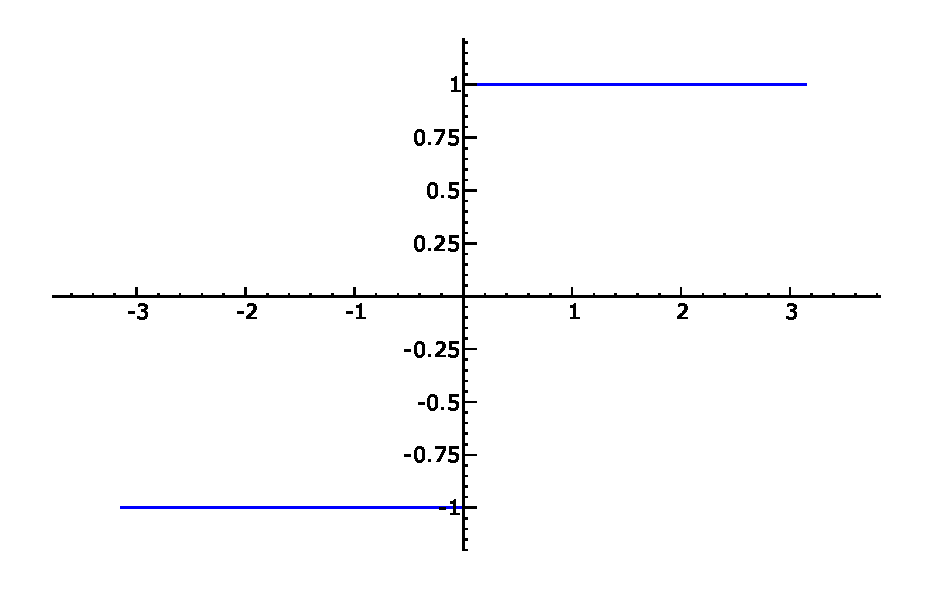
\includegraphics[width=\textwidth]{img/9April2008stepFunction.eps}
  \end{center} 
  \caption[Step Function]{Step function that we make
    periodic.}
  \label{fig:9April2008:stepFunction}
\end{figure}
We would like to compute the Fourier series of this step
function, but observe that
\begin{equation}
\int f(\theta)d\theta = |\theta|
\end{equation}
and we previously calculated the Fourier series of this
function! Recall from Eq
\eqref{eq:2April2008:fourierSeriesAbsoluteTheta} that
\begin{equation}
|\theta| = \frac{\pi}{2} - \frac{4}{\pi}\sum^{\infty}_{n=1}\frac{\cos((2n-1)\theta)}{(2n-1)^2}.
\end{equation}
We take its derivative to find
\begin{equation}
\frac{d}{d\theta}|\theta| = \frac{4}{\pi}\sum_{n=1}\frac{\sin((2n-1)\theta)}{2n-1}
\end{equation}
and we identify it with the Fourier series of the step
function
\begin{equation}
f(\theta) = \frac{4}{\pi}\sum_{n=1}\frac{\sin((2n-1)\theta)}{2n-1}.
\end{equation}
\end{ex}
